\subsection*{Relații de echivalență. Mulțimi factor (11-Oct-1994)}

Mulțimi $\rightarrow$ aplicații (morfisme) de mulțimi $\rightarrow$ submulțimi $\rightarrow$ mulțimi factor.

\begin{definition}
O relație binară este o pereche $(A, R)$, cu $A \neq \emptyset$ și $R \subseteq A \times A$.
\end{definition}

\textbf{Exemple:}
\begin{enumerate}
    \item[(1)] $A = \mathbb{N}, \quad R = \{(x, y) \in \mathbb{N} \times \mathbb{N} \mid \exists u \in \mathbb{N} \text{ a.î. } x + u = y\}$
    \item[(2)] $A = \mathbb{N}, \quad R = \{(x, y) \in \mathbb{N} \times \mathbb{N} \mid \exists q \in \mathbb{N} \text{ a.î. } x \cdot q = y\}$
    \item[(1)'] $A = \mathbb{Z}, \quad R = \{(x, y) \in \mathbb{Z} \times \mathbb{Z} \mid \exists u \in \mathbb{Z} \text{ a.î. } x + u = y\}$
    \item[(2)'] $A = \mathbb{Z}, \quad R = \{(x, y) \in \mathbb{Z} \times \mathbb{Z} \mid \exists q \in \mathbb{N} \text{ a.î. } x \cdot q = y\}$
    \item[(3)] $A = \mathbb{R}, \quad R = \{(x, y) \in \mathbb{R} \times \mathbb{R} \mid x - y \in \mathbb{Z}\}$
    \item[(4)] $n \in \mathbb{N}^*, \quad A = \mathbb{Z}, \quad R_n = \{(x, y) \in \mathbb{Z} \mid n \mid x - y \}$
    \item[(5)] $A = \text{mulțimea dreptelor dintr-un plan euclidian}$, \\ $R = \{(d_1, d_2) \in A \times A \mid d_1 = d_2 \text{ sau } d_1 \cap d_2 = \emptyset\}$
    \item[(6)] $A \xrightarrow{f} B, \quad R_f = \{(x, y) \in A \times A \mid f(x) = f(y)\}$
\end{enumerate}

\textbf{Exemplu pentru (6):} $n \in \mathbb{N}^*$, $f: \mathbb{Z} \rightarrow \mathbb{C}$, $f(k) = \cos \frac{2k\pi}{n} + i \sin \frac{2k\pi}{n}$. Atunci $R_f = R_n$.

\begin{definition}
Fie $A \neq \emptyset$, o mulțime. O submulțime $R \subseteq A \times A$ se numește \textbf{relație binară} pe $A$.
\end{definition}

\begin{remark}
Fie $M$ o mulțime. Se numește \textbf{proprietate caracteristică} a mulțimii $M$ un criteriu ce ne permite să decidem care din afirmațiile următoare sunt adevărate:
1) $x \in M$ \quad 2) $x \notin M$. \\
$M = \{x \in M \mid p(x)\}$.
\end{remark}

Dacă $x, y \in A$ și $(x, y) \in R$ atunci notăm $x R y$. Dacă $(x, y) \notin R$ notăm $x \not R y$.

\begin{definition}
Fie $R$ o relație binară pe $A$. Spunem că relația binară este:
\begin{itemize}
    \item \textbf{reflexivă} dacă $(\forall) x \in A \implies x R x$.
    \item \textbf{simetrică} dacă $x R y \implies y R x$.
    \item \textbf{antisimetrică} dacă $x R y$ și $y R x \implies x = y$.
    \item \textbf{tranzitivă} dacă $x R y$ și $y R z \implies x R z$.
\end{itemize}
\end{definition}

\begin{definition}
O relație binară $R$ pe $A$ care este:
\begin{enumerate}
    \item reflexivă, simetrică, tranzitivă s.n. \textbf{relație de echivalență}.
    \item reflexivă, antisimetrică, tranzitivă s.n. \textbf{relație de ordine}.
    \item reflexivă, tranzitivă s.n. \textbf{relație de cvasioardine} (preordine).
\end{enumerate}
\end{definition}

\textbf{Exemplu:} $(\mathbb{Z}, \equiv \pmod n)$.

Concepte asociate relațiilor de echivalență: \textbf{clasă de echivalență} și \textbf{sistem complet de reprezentanți (transversală)}.

\begin{definition}
Fie $A \neq \emptyset$ o mulțime și o relație de echivalență pe $A$. O submulțime $\emptyset \neq C \subseteq A$ se numește \textbf{clasă de echivalență} dacă:
\begin{enumerate}
    \item $(\forall) x, y \in C \implies x \sim y$
    \item dacă $z \sim x$, $x \in A$, $x \in C \implies z \in C$
\end{enumerate}
\end{definition}

\textbf{Exemplu:} $n = 6$, $C = 6\mathbb{Z} + 1 \subset \mathbb{Z}$. \\
$R_6 = \{(x, y) \in \mathbb{Z} \times \mathbb{Z} \mid 6 \mid x - y\}$
\begin{enumerate}
    \item $x, y \in C \implies 6 \mid x - y$
    \item $z \equiv x \pmod 6 \implies z - x = 6q_1$. Știind că $x = 6q + 1$, obținem: \\
    $z - (6q + 1) = 6q_1 \implies z = 6(q + q_1) + 1 \in C$.
\end{enumerate}

Fie $(A, R)$ și $a \in A$. Notăm $[a]_R = \hat{a} = C_a = \{x \in A \mid x \sim a\} \subseteq A$.

\begin{proposition}
\begin{enumerate}
    \item $\hat{a}$ este clasă de echivalență.
    \item Dacă $C \subseteq A$ este clasă de echivalență, atunci $C = [a]_R \quad (\forall) a \in C$.
\end{enumerate}
\end{proposition}

\begin{proof}
1) $\emptyset \neq C_a$ deoarece $a \in C_a$ (din reflexivitate $a \sim a$). \\
$(\forall) x, y \in C_a \implies x \sim a$ și $y \sim a \implies x \sim y$ (din simetrie și tranzitivitate). \\
Presupunem $z \sim x$, $z \in A$, $x \in C_a \implies x \sim a \implies z \sim a \implies z \in C_a$.

2) ``$\subseteq$'': Fie $x \in C$. Cum $a \in C$, avem $x \sim a \implies x \in C_a \implies C \subseteq C_a$ (clasa de echivalență a lui $a$). \\
``$\supseteq$'': Fie $x \in C_a \implies x \sim a$. Cum $a \in C$, obținem $x \in C \implies C_a \subseteq C$.
\end{proof}

\begin{proposition}
Fie $(A, R)$, $R$ o relație de echivalență.
\begin{enumerate}
    \item Pentru $a, b \in A$ avem $\hat{a} = \hat{b} \iff a \sim b$.
    \item Dacă $C'$ și $C''$ sunt două clase de echivalență, atunci $C' = C''$ sau $C' \cap C'' = \emptyset$.
\end{enumerate}
\end{proposition}


\begin{proof}
(1)
``$\implies$'': $\hat{a} = \hat{b} \implies a \in \hat{a} \implies a \in \hat{b} \implies a \sim b$. \\
``$\impliedby$'': $a \sim b \overset{?}{\implies} \hat{a} = \hat{b}$. \\
``$\subseteq$'': Fie $x \in \hat{a} \implies x \sim a$. Cum $a \sim b \implies x \sim b \implies x \in \hat{b}$. \\
``$\supseteq$'': Analoagă (idem).

(2) Fie $c \in C' \cap C'' \implies C' = \hat{c} = C''$.
\end{proof}

\begin{definition}
Fie $(A, R)$ cu $A \neq \emptyset$ și $R$ o relație de echivalență. O familie de elemente din $A$ se numește \textbf{sistem complet de reprezentanți} (S.C.R.) dacă:
\begin{itemize}
    \item[$(\alpha)$] $(\forall) i, j \in I, i \neq j \implies a_i \not\sim a_j$
    \item[$(\beta)$] $(\forall) x \in A, \exists! i \in I \text{ a.î. } x \sim a_i$
\end{itemize}
\end{definition}

\textbf{Exemple:}
\begin{enumerate}
    \item $(\mathbb{Z}, R_6)$, mulțimea $\{0, 1, 2, 3, 4, 5\} \subset \mathbb{Z}$ este un sistem complet de reprezentanți pentru $R_6$. \\
    $x \in \mathbb{Z} \implies x = 6q + r, \quad 0 \leq r < 6$. \\
    Mulțimea $\{6q, 1+6q, \dots, 5+6q\}$ este, de asemenea, un S.C.R. \\
    $x - r \text{ este multiplu de } 6 \implies x \equiv r \pmod 6$.
    \item $A = \mathbb{R}$. Intervalul $[0, 1) \subset \mathbb{R}$, iar $R = \{(x, y) \in \mathbb{R} \times \mathbb{R} \mid x - y \in \mathbb{Z}\}$. \\
    $x \in \mathbb{R} \implies \exists! a \in [0, 1) \text{ a.î. } x - a \in \mathbb{Z}$. \\
    $x = [x] + \{x\}$, unde $a = \{x\} \in [0, 1) \implies [0, 1)$ este un sistem complet de reprezentanți.
\end{enumerate}

\begin{definition}
Fie $(A, R)$, cu $R$ o relație de echivalență. Mulțimea:
$$ \frac{A}{R} = \{\hat{a} \mid a \in A\} $$
reprezintă mulțimea tuturor claselor de echivalență și se numește \textbf{mulțimea factor} a lui $A$ prin $R$.
\end{definition}

\begin{proposition}
$\frac{A}{R} = \{\hat{a}_i \mid i \in I\}$ unde $\{a_i\}_{i \in I}$ este un sistem complet de reprezentanți. \\
$(\forall) a \in A, \exists a_i$ a.î. $\hat{a} = \hat{a}_i$.
\end{proposition}

\textbf{Exemple:}
$\frac{\mathbb{Z}}{R_6} = \{\hat{0}, \hat{1}, \hat{2}, \hat{3}, \hat{4}, \hat{5}\}$. În general, $\frac{\mathbb{Z}}{R_n} = \{\hat{0}, \hat{1}, \dots, \widehat{n-1}\}$.

\begin{remark}
Dacă $\{a_i\}_{i \in I} \subset A$ este o transversală în $A$ pentru o relație de echivalență $R$, atunci:
$$ A = \bigcup_{i \in I} \hat{a}_i \quad \text{(reuniune disjunctă)} $$
\end{remark}

\begin{proof}
``$\supseteq$'': Evident. \\
``$\subseteq$'': Folosim punctul $(\beta)$ din definiția sistemului complet de reprezentanți. \\
Fie $x \in A \implies \exists i \in I \text{ a.î. } x \sim a_i \implies x \in \hat{a}_i \implies x \in \bigcup_{i \in I} \hat{a}_i$. \\
Reuniunea este disjunctă pentru că $\hat{a}_i \cap \hat{a}_j = \emptyset$ pentru $i \neq j$.
\end{proof}

\textbf{Exemplu:} $\mathbb{Z} = 6\mathbb{Z} \cup (6\mathbb{Z}+1) \cup \dots \cup (6\mathbb{Z}+5)$.

\begin{definition}
O \textbf{partiție} a unei mulțimi $A \neq \emptyset$ este o familie de submulțimi $A_i \subset A$, $A_i \neq \emptyset$, astfel încât:
\begin{itemize}
    \item $i \neq j \implies A_i \cap A_j = \emptyset$
    \item $\bigcup_{i \in I} A_i = A$
\end{itemize}

% Diagrama partiției
\begin{center}
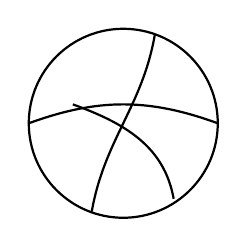
\begin{tikzpicture}[scale=0.8]
  \draw[thick] (0,0) circle (1.5cm);
  \draw[thick] (-1.5,0) to[out=20,in=160] (1.5,0);
  \draw[thick] (-0.5,-1.4) to[out=80,in=260] (0.5,1.4);
  \draw[thick] (-0.8,0.3) to[out=-20,in=100] (0.8,-1.2);
\end{tikzpicture}
\end{center}
\end{definition}

Pe o mulțime $A$ putem defini atâtea relații de echivalență câte partiții putem stabili pentru $A$.
Dacă avem o partiție, definim relația: $x, y \in A \implies \left( x \sim y \overset{\text{def}}{\iff} \exists i \text{ a.î. } x, y \in A_i \right)$.

\textbf{Exercițiu:} Câte relații de echivalență pot fi definite pe o mulțime cu 6 elemente?

\begin{definition}
Fie $(A, R)$, cu $R$ o relație de echivalență. Definim funcția:
$$ p : A \rightarrow \frac{A}{R}, \quad p(a) = \hat{a} $$
Funcția $p$ este surjectivă și se numește \textbf{aplicația canonică} a mulțimii factor. Imaginea inversă a unui element din mulțimea factor este o clasă de echivalență.
\end{definition}

\textbf{Exemplu:} $p: \mathbb{Z} \rightarrow \frac{\mathbb{Z}}{R_n} = \mathbb{Z}_n, \quad p(x) = \hat{x} = n\mathbb{Z} + x$.

\begin{theorem}[Teorema de factorizare pentru o aplicație de mulțimi]
(Aplicația indusă pe o mulțime factor de către o aplicație de mulțimi). \\
Dacă $f: A \rightarrow B$ este o funcție compatibilă cu relația de echivalență $R$, atunci $\exists f^* : \frac{A}{R} \rightarrow B$ astfel încât triunghiul următor să fie comutativ ($f = f^* \circ p$).

\begin{center}
\begin{tikzcd}[row sep=large, column sep=large]
A \arrow[r, "f"] \arrow[d, "p"'] & B \\
A/R \arrow[ur, dashed, "f^*"'] &
\end{tikzcd}
\hspace{2cm}
\begin{tikzcd}[row sep=large, column sep=large]
a \arrow[r, mapsto] \arrow[d, mapsto] & f(a) \\
\hat{a} \arrow[ur, mapsto] &
\end{tikzcd}
\end{center}
\end{theorem}

\begin{remark}
Dacă funcția $f^*$ există, ea este unică. Dacă $f_1^* \circ p = f_2^* \circ p$, deoarece $p$ este surjectivă (epimorfism), rezultă $f_1^* = f_2^*$.
\end{remark}